%% Author: thompson
%% 26.10.17
%%

% Preamble
\documentclass[11pt]{article}

% Packages
\usepackage{a4wide}
\usepackage[utf8]{inputenc}     % Enables ö ä ü
\usepackage[ngerman]{babel}     % Deutsche Rechtschreibung @ Long words
\usepackage{graphicx}           % Graphic-Imports

% Document
\begin{document}

    \section{Netzwerktypen}
    \subsection{Leitungsvermittelnde Netzwerke}
    Leitungsvermittelnde Netzwerke, oder Circuit-Switch Networks, sind vergleichbar mit Telefonanrufen oder einem Schienennetz. Ein exklusiver logischer oder physikalischer
    Pfad wird zwischen Sender und Empfänger designiert, vergleichbar mit einer Krititschen Zone. Genutzte
    Ressourcen, benutzt oder nicht, stehen in dieser Zeit anderen Usern nicht zur Verfügung. Problematik: Leitungsblockierung\\

        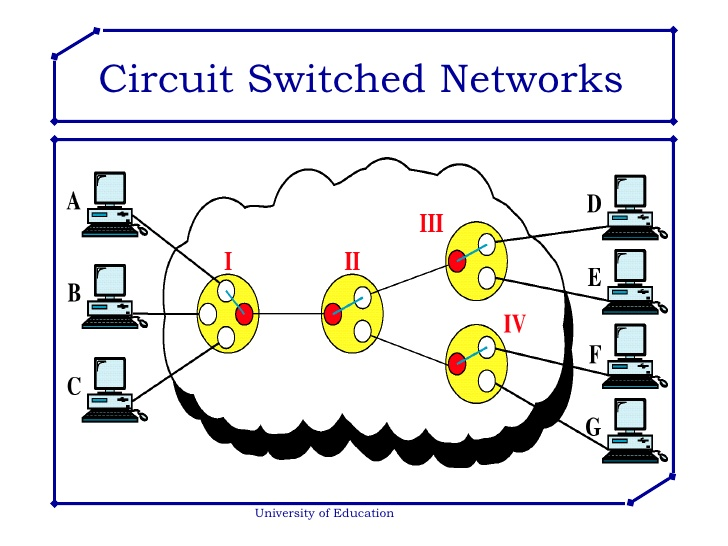
\includegraphics[width=\textwidth]{Circuit_SwitchNetwork.jpg}

    \subsection{Paketvermittelnde Netzwerke}
    Paketvermittelnde Netzwerke, oder Packet-Switching Networks, sind charakteristisch gesehen wie E-Mails. Daten werden Bufferähnlich zu einem größeren Datensatz zusammengeschrieben,
    welches das Datenpaket ausmacht. Diese werden vollständig gesendet \& vollständig empfangen, wobei
    die Pakete über dynamisch bestehende Pfade via Nodes verschickt wird. Dies ermöglicht parallelen Transfer zwischen
    mehreren Usern und erhöht die Ausfallsicherheit, da die Zielpfade der Pakete zur Laufzeit veränderbar sind. "Store and Forward"-Prinzip bei 1500 Byte <=> Maximum Transfer Unit.\\

        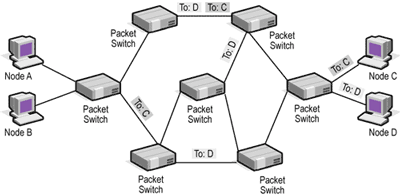
\includegraphics[width=\textwidth]{PacketSwitching_Networks.png}

\end{document}